\begin{enumerate}[label=\thechapter.\arabic*,ref=\thechapter.\theenumi]
\numberwithin{equation}{enumi}
\numberwithin{figure}{enumi}
\numberwithin{table}{enumi}
\item Let
\begin{align}
	X=\text{Bin}(n,p).
\end{align}
The mean and variance are then given by 
\begin{align}
    \mu = np,\,
    \sigma^2 = npq.
\end{align}
\item For large values of $n,k, n-k$, by Stirling's Approximation.
\begin{align}
\begin{split}
    n! &\approx n^n e^{-n} \sqrt{2\pi n}
    \\
    k! &\approx k^k e^{-k} \sqrt{2\pi k}
    \\
	\brak{n-k}! &\approx \brak{n-k}^{\brak{n-k}} e^{-\brak{n-k}} \sqrt{2\pi \brak{n-k}}
\end{split}
  \label{eq:ncert/12/13/6/4/1/stirling}
\end{align}
\item Then, 
\begin{align}
	p_X(k ) &= \frac{n!}{k!(n-k)!}p^kq^{n-k}
    \approx \frac{n^n e^{-n} \sqrt{2\pi n}}{k^k e^{-k} \sqrt{2\pi k} (n-k)^{n-k} e^{-(n-k)} \sqrt{2\pi (n-k)}} p^k q^{n-k}\\
    &= \brak{\frac{np}{k}}^k \brak{\frac{nq}{n-k}}^{n-k} \sqrt{\frac{n}{2\pi k(n-k)}}
  \label{eq:ncert/12/13/6/4/1/stirling/pmf}
\end{align}
from 
  \eqref{eq:ncert/12/13/6/4/1/stirling}
\item For
\begin{align}
	\delta \ll np, nq, 
  \label{eq:ncert/12/13/6/4/1/delta/approx}
\end{align}
and 
\begin{align}
	k &= np + \delta,
	\\
	n-k &= nq -\delta
	\\
	\implies 
\begin{split}
	\frac{k}{np} &= 1 + \frac{\delta}{np}
	\\
	\frac{n-k}{nq} &= 1 - \frac{\delta}{nq}
\end{split}
  \label{eq:ncert/12/13/6/4/1/delta}
\end{align}
\item Taking logarithms in
  \eqref{eq:ncert/12/13/6/4/1/stirling/pmf},
\begin{align}
	\ln\sbrak{	p_X(k )} 
	&= -k\ln\brak{\frac{np}{k}}- \brak{n-k}\brak{\frac{nq}{n-k}} + \frac{1}{2}\ln\brak{\frac{n}{2\pi k(n-k)}}
	\\
	&= -\brak{np+\delta}\ln\brak{1+\frac{\delta}{np}}  -\brak{nq-\delta}\brak{1-\frac{\delta}{nq}} 
	\nonumber \\
	&\quad + \frac{1}{2}\ln\brak{\frac{n}{2\pi \brak{np+\delta}\brak{nq-\delta}}}
  \label{eq:ncert/12/13/6/4/1/stirling/pmf/log}
\end{align}
upon substituting from 
  \eqref{eq:ncert/12/13/6/4/1/delta}.
  From 
  \eqref{eq:ncert/12/13/6/4/1/delta/approx},
\begin{align}
	 \frac{1}{2}\ln\brak{\frac{n}{2\pi \brak{np+\delta}\brak{nq-\delta}}} \approx 
	 \frac{1}{2}\ln\brak{\frac{1}{2\pi npq}}  
  \label{eq:ncert/12/13/6/4/1/stirling/sqrt}
\end{align}
  From 
  \eqref{eq:ncert/12/13/6/4/1/delta/approx}
  and the approximation
\begin{align}
    \ln{\brak{1+x}} \approx x-\frac{x^2}{2},
\end{align}
 the first sum in  \eqref{eq:ncert/12/13/6/4/1/stirling/pmf/log} can be expressed as,
  \begin{multline}
	 -\brak{np+\delta}\ln\brak{1+\frac{\delta}{np}}  -\brak{nq-\delta}\brak{1-\frac{\delta}{nq}} 
	\\
	\approx
    -( np+\delta )\brak{\frac{\delta}{np}-\frac{\delta^2}{2n^2 p^2}}
    -(nq-\delta)\brak{-\frac{\delta}{nq}-\frac{\delta^2}{2n^2q^2}}
    \\
    =-\delta \sbrak{1+\frac{\delta}{2np}-1+\frac{\delta}{2nq}}
    = - \frac{\delta^2}{2npq}
  \label{eq:ncert/12/13/6/4/1/stirling/sum}
    %\\brak{\frac{np}{k}}^k \brak{\frac{nq}{n-k}}^{(n-k)}&=e^{-\frac{\delta^2}{2npq}}
  \end{multline}
  Substituting from 
  \eqref{eq:ncert/12/13/6/4/1/stirling/sum}
  and
  \eqref{eq:ncert/12/13/6/4/1/stirling/sum}
  in 
  \eqref{eq:ncert/12/13/6/4/1/stirling/pmf/log},
\begin{align}
	\ln\sbrak{	p_X(k )} 
     &\approx 
	 \frac{1}{2}\ln\brak{\frac{1}{2\pi npq}}  
- \frac{\delta^2}{2npq}
\\
\implies
	p_X(k )&=
	\sqrt{\frac{1}{2\pi npq}} e^{-\frac{(k-np)^2}{2npq}}
     =\frac{1}{\sigma\sqrt{2\pi}}e^{-\frac{(k-\mu)^2}{2\sigma^2}}
\end{align}
\item A comparison of Binomial and Gaussian pmf/pdf is provided in 
	Figs. 
  \ref{fig:ncert/12/13/6/4/1}
  and
  \ref{fig:ncert/12/13/6/4/2}.
\begin{figure}[h]
%\begin{subfigure}{0.4\textwidth}
  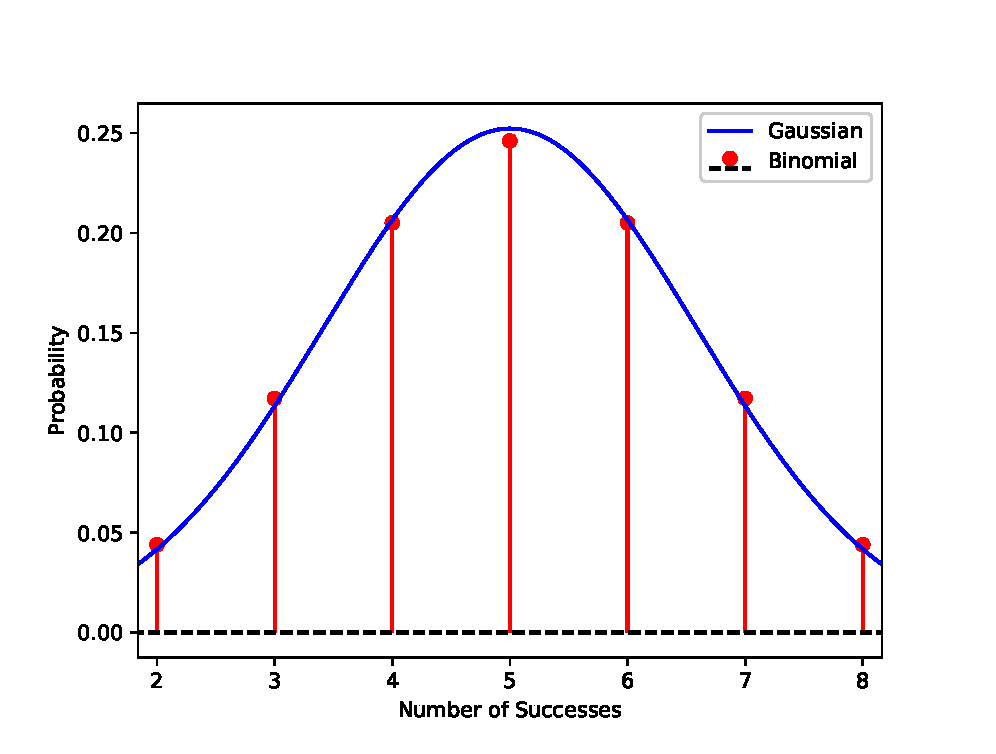
\includegraphics[width=\columnwidth]{ncert/12/13/6/4/figs/10.eps}
  \caption{10 trials}
  \label{fig:ncert/12/13/6/4/1}
\end{figure}
%\end{subfigure}
%\begin{subfigure}{0.4\textwidth}
\begin{figure}[h]
  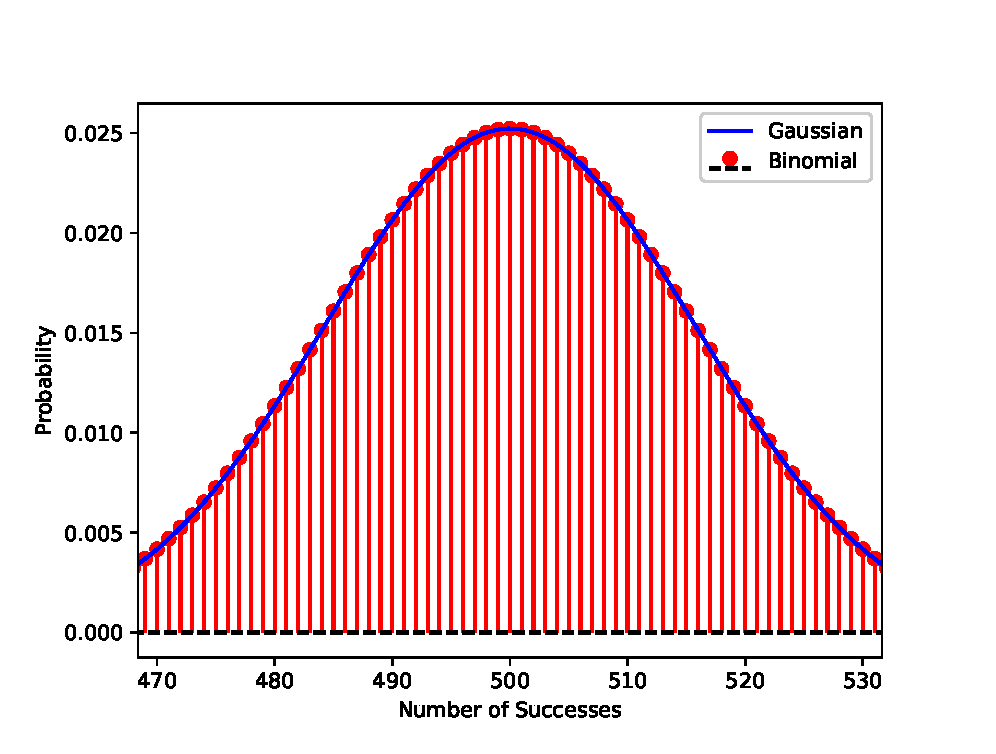
\includegraphics[width=\columnwidth]{ncert/12/13/6/4/figs/1000.eps}
  \caption{1000 trails}
  \label{fig:ncert/12/13/6/4/2}
%\end{subfigure}
\end{figure}
\end{enumerate}
